\centering
\begin{tikzpicture}[node distance=1.5cm]

	\rootnode;
	
	\proofnode[above right of=root]{ghost}{};
	\proofnode[above left of=root]{n6}{$\{x_3\}$};
	\proofnode[above right of=ghost]{n8}{$\{\neg x_3\}$};
	\drawchildren{root}{n6}{n8};
	\withchildren{n6}{n3}{$\{\neg x_2,x_3\}$} {n5} {$\{\neg x_2\}$};
	\withchildren{n3}{n1}{$\{x_1,x_2,\neg x_3\}$} {n2} {$\{\neg x_1\}$};
	\proofnode[above right of=n5]{n4} {$\{x_1,\neg x_2\}$};
	\drawchildren{n5}{n2}{n4};
	
	\proofnode[above right of=n8]{n7} {$\{x_1,\neg x_3\}$};
	\drawchildren{n8}{n7}{n2};
	
\end{tikzpicture}
